\SourcePage{21}
\SGAsection{2}{意大利学派的交点理论}
设 $S'$ 和 $S$ 是域 $k$ 上的两个\Term{smooth}{光滑}\Term{projective-surface}{射影曲面}，$f:S'\to S$ 是\Term{birational-morphism}{双有理态射}。若 $D,E$ 是 $S$ 上的两个\Term{divisor}{除子}，则
\[
(D,E)=(f^*D,f^*E).
\]
\SourcePage{22}
例如，移动 $D,E$ 即可看出这一点。

因此，自然要给\Term{intersection-number}{交数}一个“\Term{birational}{双有理}”的表达式。这里要说明意大利学派为此所用的方法。我的主要资料来源是 [1]，其中有很长的参考书目。另见 Manin [6] 和 Northcott [12]、[13]。

\textbf{(2.0)} 设 $S$ 是二维\Term{regular-local-ring}{正则局部环}的\Term{spectrum}{谱}，$s$ 是其\Term{closed-point}{闭点}，$k$ 是 $k(s)$ 的一个子域，且 $k(s)/k$ 是\Term{finite-extension}{有限扩张}。\Term{intersection-number}{交数}及 Euler--Poincaré \Term{euler-poincare-characteristic}{示性数}均相对于 $k$ 计算。

本节称一个 $S$-\Term{scheme}{概形} $p:S'\to S$ 为 $S$ 的\Term{birational-transform}{双有理变换}，如果 $S'$ \Term{regular}{正则}、\Term{connected}{连通}，$p$ \Term{proper}{固有}，且在 $S'\setminus p^{-1}(s)$ 与 $S\setminus\{s\}$ 之间诱导\Term{isomorphism}{同构}。关于 $S$ 的一切论述，也适用于其\Term{birational-transform}{双有理变换}在\Term{closed-point}{闭点}处的\Term{localization}{局部化}。

\textbf{(2.1)} 设 $f:(S'',p'')\to(S',p')$ 是 $S$ 的\Term{birational-transform}{双有理变换}之间的一个 $S$-\Term{morphism}{态射}。已知 [5]，$f$ 有且仅有一个\Term{resolution}{分解}
\[
f=f_n\cdots f_1,\qquad f_i:S_{i+1}\longrightarrow S_i,
\]
使 $S_{i+1}$ 由 $S_i$ 沿一个\Term{finite}{有限}\Term{closed-point}{闭点}集 $X_i$ \Term{blow-up}{爆破}而得，并且 $f_i(X_{i+1})\subset X_i$。$X_i$ 正是 $S_i$ 上使 $S''$ 到 $S_i$ 的\Term{projection}{投影}不是\Term{isomorphism}{同构}的那些点的\Term{set}{集合}。

特别地，$f$ 在 $S'$ 的某个\Term{finite}{有限}\Term{subset}{子集}的补集上诱导\Term{isomorphism}{同构}，而该补集包含 $p'^{-1}(s)$ 各\Term{irreducible-component}{不可约分支}的\Term{generic-point}{一般点}。因此 $f^{-1}$ 给出一个\Term{injectivity}{单射}，把 $p'^{-1}(s)$ 的\Term{irreducible-component}{不可约分支}集
\SourcePage{23}
$\operatorname{Irr}(p'^{-1}(s))$ 映入 $\operatorname{Irr}(p''^{-1}(s))$。

$S$ 的\Term{birational-transform}{双有理变换}没有非恒等的 $S$-\Term{automorphism}{自同构}。以下用 $I$ 表示这些\Term{birational-transform}{双有理变换}的 $S$-\Term{isomorphism}{同构}类的\Term{set}{集合}，按\Term{domination}{支配}关系排序。$I$ 是\Term{filtered}{右滤过}的，且有最小元 $S$。

\begin{SGAresult}{定义}{2.2}
$S$ 中与 $s$ \Term{infinitely-near-point}{无穷邻近的点}所成的\Term{set}{集合} $S^*$，定义为\Term{inductive-limit}{归纳极限}
\[
S^*=\varinjlim_I\operatorname{Irr}(p^{-1}(s)).
\]
\end{SGAresult}
若 $t\in S^*$ 在 $S$ 的一个\Term{birational-transform}{双有理变换} $S'$ 上由一条\Term{complete-curve}{完备}、\Term{reduced}{约化}、\Term{irreducible}{不可约}\Term{curve}{曲线} $T$ 表示，则域 $H^0(T,\mathcal O_T)$ 只依赖于 $t$，与 $S'$ 的选择无关；称之为 $t$ 的\Term{residue-field}{剩余域} $k(t)$。

设 $S_1$ 是 $S$ 沿 $s$ 的\Term{blow-up}{爆破}。$\{s\}$ 在 $S_1$ 中的\Term{inverse-image}{逆像}是\Term{projective-line}{射影直线} $s^*$，称为 $s$ 的\Term{curvetta}{小曲线（curvetta）}；它确定 $S^*$ 的一个元素 $s^*$，其\Term{residue-field}{剩余域}为 $k(s)$。

设 $S'$ 是 $S$ 的一个\Term{birational-transform}{双有理变换}，$t$ 是 $S'$ 的一个\Term{closed-point}{闭点}，$S'_t$ 是 $S'$ 在 $t$ 处的\Term{local-ring}{局部环}的\Term{spectrum}{谱}。显然可定义一个从 $S_t'^*$ 到 $S^*$ 的\Term{injectivity}{单射}；特别地，$t$ 确定一个元素 $t^*\in S^*$，二者\Term{residue-field}{剩余域}相同。用 $S'^*$ 表示所有 $S_t'^*$ 在 $S^*$ 中的并，其中 $t$ 遍历 $S'$ 的\Term{closed-point}{闭点}。

下述命题由 2.1 对 $S$ 的\Term{birational-transform}{双有理变换}的描述得到。
\SourcePage{24}
\begin{SGAresult}{命题}{2.3}
对任意 $t\in S^*$，恰有一个由 $S$ 的\Term{birational-transform}{双有理变换}组成的序列 $(S_i)_{0\leq i\leq n+1}$，及\Term{closed-point}{闭点} $t_i\in S_i$（$0\leq i\leq n$），满足：
\begin{enumerate}
\item[(i)] $S_0=S$，且 $S_{i+1}$ 是 $S_i$ 沿 $\{t_i\}$ 的\Term{blow-up}{爆破}；
\item[(ii)] $t_{i+1}\in t_i^*$（$0\leq i<n$），且 $t=t_n^*$。
\end{enumerate}
此外，对 $S$ 的任意\Term{birational-transform}{双有理变换} $(S',p')$，$t$ 属于 $\operatorname{Irr}(p'^{-1}(s))$ 在 $S^*$ 中的像，当且仅当 $S'$ \Term{domination}{支配} $S_{n+1}$。
\end{SGAresult}
称 $n$ 为 $t$ 的\Term{order-near-point}{阶}。这里用 $S(t)$（分别用 $S_+(t)$）表示 $S$ 的\Term{birational-transform}{双有理变换} $S_n$（分别为 $S_{n+1}$）。稍滥用记号，仍以 $t$ 表示 $S_n$ 的\Term{closed-point}{闭点} $t_n$，并以 $t^*$ 表示它在 $S_{n+1}$ 中的\Term{inverse-image}{逆像} $t_n^*$。

赋予 $S^*$ 如下的序：
\[
t_1\prec t_2\quad\Longleftrightarrow\quad S_+(t_2)\text{ 支配 }S_+(t_1).
\]
若 $t_1\prec t_2$，则 $k(t_2)$ 是 $k(t_1)$ 的\Term{group-extension}{扩张}。\Term{ordered-set}{有序集} $S^*$ 有最小元 $s^*$，且每个有上界的\Term{subset}{子集}都是\Term{finite}{有限}\Term{totally-ordered}{全序集}（$S^*$ 是一棵“以 $s^*$ 为根的树”）。此外，$t\in S^*$ 的\Term{order-near-point}{阶} $n$ 就是树 $S^*$ 中从 $s^*$ 到 $t$ 的距离（$n=\#[s^*,t]$）。

下述命题明确给出 2.1 对 $S$ 的\Term{birational-transform}{双有理变换}的描述。
\begin{SGAresult}{命题}{2.4}
把 $S$ 的一个\Term{birational-transform}{双有理变换} $p:S'\to S$ 映为 $S^*$ 的\Term{subset}{子集} $\operatorname{Irr}(p^{-1}(s))$ 的映射，在\Term{set}{集合} $I$（2.1）与 $S^*$ 中下述\Term{finite}{有限}\Term{subset}{子集}的\Term{set}{集合}之间诱导\Term{bijection}{双射}：这些\Term{subset}{子集}每包含一个元素，
\SourcePage{25}
便也包含其所有前驱。
\end{SGAresult}
设 $D$ 是 $S$ 上的一个\Term{effective-divisor}{有效除子}，$t\in S^*$。若 $S(t)$（2.3）的\Term{closed-point}{闭点} $t$ 属于 $D$ 在 $S(t)$ 上的\Term{strict-transform}{严格变换}（即 $D\setminus\{s\}$ 的\Term{schematic-closure}{概形论闭包}），就说 $t$ 属于 $D$。

\begin{SGAresult}{定义}{2.5}
设 $t,t'\in S^*$。若 $t'\in S_+(t)^*$（2.2），且 $t'$ 属于 $t$ 的\Term{curvetta}{小曲线} $t^*$（2.3），则称 $t'$ \Term{proximate-point}{邻近} $t$。
\end{SGAresult}
若 $t'$ 是 $t$ 的直接后继，则 $t'$ \Term{proximate-point}{邻近} $t$；若序列 $(t_i)_{0\leq i\leq n}$ 中的每个 $t_{i+1}$ 都是 $t_i$ 的直接后继，而 $t_n$ \Term{proximate-point}{邻近} $t_0$，则对 $0<i\leq n$，$t_i$ 都\Term{proximate-point}{邻近} $t_0$，且 $t_n$ 不\Term{proximate-point}{邻近}任何 $t_i$（$0<i\leq n-1$）。

\textbf{(2.6)} 设 $A$ 是\Term{dimension}{维数}为 $n$ 的 Noether \Term{local-ring}{局部环}，$T$ 是其\Term{spectrum}{谱}，$\mathfrak m$ 是其\Term{maximal-ideal}{极大理想}，$k=A/\mathfrak m$ 是其\Term{residue-field}{剩余域}，$P=\sum_{0\leq i<n}a_iX^i$ 是其 Hilbert--Samuel \Term{polynomial}{多项式}：
\[
P(n)=\dim_k(\mathfrak m^n/\mathfrak m^{n+1})\qquad(n\text{ 充分大}).
\]
回忆，$T$ 的\Term{closed-point}{闭点} $s$ 的\Term{multiplicity}{重数} $\mu_s$ 按定义满足
\[
a_{n-1}=\mu_s/(n-1)!.
\]
因而当 $n=1$ 时，简单地有
\[
\mu_s=\dim_k(\mathfrak m^n/\mathfrak m^{n+1})\qquad(n\text{ 充分大}).
\]
从几何上说，$\mu_s$ 可定义为 $T$ 沿\Term{closed-subscheme}{闭子概形} $\{s\}$ 的\Term{blow-up}{爆破}的\Term{special-fibre}{特殊纤维}在 $k$ 上的\Term{projective-space}{射影空间} $\mathbb P_k(\mathfrak m/\mathfrak m^2)$ 中的\Term{degree}{次数}。
\SourcePage{26}
回忆，若 $Y,Z$ 是\Term{scheme}{概形} $X$ 的两个\Term{closed-subscheme}{闭子概形}，则 $Y$ 在 $X$ 沿 $Z$ 的\Term{blow-up}{爆破} $\widetilde X$ 中的\Term{strict-transform}{严格变换}，即 $Y\setminus Z$ 在 $\widetilde X$ 中的\Term{schematic-closure}{概形论闭包}，就是 $Y$ 沿 $Y\cap Z$ 的\Term{blow-up}{爆破}。

设 $T$ 是\Term{regular}{正则}\Term{scheme}{概形} $U$ 的一个\Term{closed-subscheme}{闭子概形}。令 $p:U_1\to U$ 为 $U$ 沿 $\{s\}$ 的\Term{blow-up}{爆破}，$s^*$ 为 $s$ 在 $U_1$ 中的\Term{inverse-image}{逆像}，$T'$ 为 $T$ 在 $U_1$ 中的\Term{strict-transform}{严格变换}。以上说明，$T$ 在 $s$ 处的\Term{multiplicity}{重数}是\Term{closed-subscheme}{闭子概形} $s^*\cap T'$ 在\Term{projective-space}{射影空间} $s^*$ 中的\Term{degree}{次数}。

再设 $T$ 是 $U$ 的\Term{divisor}{除子}，记其在 $U_1$ 中的\Term{total-transform}{全变换}（即\Term{inverse-image}{逆像}\Term{divisor}{除子}）为 $T^*$，并用公式 $T^*=\nu s^*+T'$ 定义 $\nu$。若 $X$ 是 $s^*$ 中的一条直线，且 Euler--Poincaré \Term{euler-poincare-characteristic}{示性数}按 $k$ 上\Term{dimension}{维数}的\Term{alternating-sum}{交错和}计算，则已知
\[
(X,s^*)=\chi(\mathcal O_X\mathbin{\otimes^{\mathbf L}}\mathcal O_{s^*})=\deg_X\mathcal O(s^*)=-1,\tag{2.6.1}
\]
并且已经验证
\[
(X,T')=\chi(\mathcal O_X\mathbin{\otimes^{\mathbf L}}\mathcal O_{T'})=\deg_{s^*}(s^*\cap T')=\mu_s.\tag{2.6.2}
\]
\Term{projection-formula}{投影公式}
\[
Rp_*(\mathcal O_X\mathbin{\otimes^{\mathbf L}}\mathcal O_{T^*})
=Rp_*(\mathcal O_X\mathbin{\otimes^{\mathbf L}}Lp^*\mathcal O_T)
=Rp_*\mathcal O_X\mathbin{\otimes^{\mathbf L}}\mathcal O_T
\]
及其推论
\[
(X,T^*)=\nu(X,s^*)+(X,T')=0
\]
结合 (2.6.1)、(2.6.2)，给出恒等式
\[
\mu_s=\nu.\tag{2.6.3}
\]
\SourcePage{27}
\begin{SGAresult}{命题}{2.7}
设 $T$ 是\Term{regular}{正则}\Term{scheme}{概形} $U$ 中的一个\Term{effective-divisor}{有效除子}，$s$ 是 $U$ 的一个\Term{closed-point}{闭点}，$U_1$ 是 $U$ 沿 $\{s\}$ 的\Term{blow-up}{爆破}，$s^*$ 是 $s$ 在 $U_1$ 中的\Term{inverse-image}{逆像}，$T'$ 是 $T$ 在 $U_1$ 上的\Term{strict-transform}{严格变换}，$T^*$ 是其\Term{total-transform}{全变换}。以下三个数相同：
\begin{enumerate}
\item[(i)] $T$ 的点 $s$ 在 Samuel 意义下的\Term{multiplicity}{重数}；
\item[(ii)] $s^*\cap T'$ 在\Term{projective-space}{射影空间} $s^*$ 中的\Term{degree}{次数}；
\item[(iii)] $s^*$ 在\Term{divisor}{除子} $T^*$ 中的\Term{multiplicity}{重数}。
\end{enumerate}
\end{SGAresult}
\textbf{2.8.} 回到 2.0 的假设。设 $D$ 是 $S$ 上的\Term{effective-divisor}{有效除子}，$t\in S^*$。$D$ 在 $t$ 处的\Term{multiplicity}{重数} $\mu_t(D)$ 按定义是 $D$ 在 $S(t)$（2.3）上的\Term{strict-transform}{严格变换}在 $t$ 处的\Term{multiplicity}{重数}。函数 $t\mapsto\mu_t(D)$ 的\Term{support}{支集}是属于 $D$ 的、与 $s$ \Term{infinitely-near-point}{无穷邻近的点}的\Term{set}{集合}（2.4）。当 $D$ \Term{regular}{正则}时，数 $\mu_t(D)[k(t):k(s)]$ 等于零或一：事实上，$D$ 的各\Term{strict-transform}{严格变换} $D'$ 都与 $D$ \Term{isomorphism}{同构}，然后应用\Term{multiplicity}{重数}的定义 (2.6) 即可。

\Term{intersection-number}{交数}可用\Term{multiplicity}{重数}来计算：
\begin{SGAresult}{\Term{theorem}{定理}}{2.9}
若\Term{divisor}{除子} $D,E$ 只在 $s$ 相交，则
\[
(D,E)=\sum_{t\in S^*}\mu_t(D)\mu_t(E)[k(t):k],
\]
求和遍历 $D,E$ 共有的、与 $s$ \Term{infinitely-near-point}{无穷邻近的点}。
\end{SGAresult}
\begin{proof}
设 $p:S'\to S$ 是 $S$ 的\Term{birational-transform}{双有理变换}。用 $D^*,E^*$（分别用 $D',E'$）表示 $D,E$ 的\Term{total-transform}{全变换}（分别为\Term{strict-transform}{严格变换}）。
\SourcePage{28}
\begin{SGAresult}{\Term{lemma}{引理}}{2.9.1}
\begin{enumerate}
\item[(i)] \Term{total-transform}{全变换} $D^*$ 由下列条件刻画：
\begin{enumerate}
\item[(a)] $D^*-D'$ 集中在 $f^{-1}(s)$ 上；
\item[(b)] 若 $X$ 集中在 $f^{-1}(s)$ 上，则 $(D^*,X)=0$。
\end{enumerate}
\item[(ii)] $(D,E)=(D^*,E^*)=(D^*,E')=(D',E^*)$。
\end{enumerate}
\end{SGAresult}
断言 (i)(a) 显然，而 (i)(b) 由 1.6 (vi) 得到。条件 (a)、(b) 确定 $D^*$，这是 1.9 的结论。由构造，$\mathcal O_E\to f_*\mathcal O_{E'}$ 的\Term{cokernel}{余核}是\Term{finite}{有限}的，从而
\[
(D^*,E')=\chi(f^*\mathcal O_D\otimes\mathcal O_{E'})
=\chi(\mathcal O_D\otimes f_*\mathcal O_{E'})
=\chi(\mathcal O_D\otimes\mathcal O_E)=(D,E),
\]
再由 (i) 即得 (ii)。

取 $S'$ 为 $S$ 在 $s$ 处的\Term{blow-up}{爆破}。由 (2.9.1)、(2.6.3) 和 2.7，
\begin{align}
(D,E)&=(D^*,E')=(D'+\mu_s(D)s^*,E')\notag\\
&=(D',E')+\mu_s(D)(s^*,E')\notag\\
&=(D',E')+\mu_s(D)\mu_s(E)[k(s):k].\tag{2.9.2}
\end{align}
现在对 $(D,E)$ 归纳，反复应用 (2.9.2)，便证明了\Term{theorem}{定理} 2.9。
\end{proof}

\textbf{(2.10)} 设 $A$ 是一维 Noether \Term{reduced}{约化}\Term{local-ring}{局部环}，$s$ 是 $\operatorname{Spec}(A)$ 的\Term{closed-point}{闭点}，$\widetilde A$ 是 $A$ 的\Term{normalization}{正规化}，$k$ 是一个域，且 $k(s)/k$ 为\Term{finite-extension}{有限扩张}。设 $\widetilde A$ 在 $A$ 上\Term{finite}{有限}（即\Term{completion}{完备化} $\widehat A$ \Term{reduced}{约化}）。把 $A$-模 $\widetilde A/A$ 相对于 $k$ 计算的\Term{length}{长度}，称为 $\operatorname{Spec}(A)$ 在 $s$ 处的\Term{delta-invariant}{奇点的 $\delta$ 不变量}。
\SourcePage{29}
\begin{SGAresult}{\Term{theorem}{定理}}{2.11}
设 $D$ 是 $S$ 上的一条\Term{reduced}{约化}\Term{curve}{曲线}。则：
\begin{enumerate}
\item[(i)] 对任意 $t\in S^*$，采用 2.8 的记号，有
\[
\mu_t(D)=\sum_{t'\text{ 邻近 }t}\mu_{t'}(D)[k(t'):k(t)].
\]
\item[(ii)] 设 $D$ 的\Term{normalization}{正规化} $\widetilde D$ 在 $D$ 上\Term{finite}{有限}，$\delta=\chi(\mathcal O_{\widetilde D}/\mathcal O_D)$ 是 $D$ 在 $s$ 处的\Term{delta-invariant}{奇点不变量}。除\Term{finite}{有限}多个 $t\in S^*$ 外，$\mu_t(D)$ 都等于零或一，并且
\[
\delta=\sum_{t\in S^*}\frac12\mu_t(D)(\mu_t(D)-1)[k(t):k].
\]
\end{enumerate}
\end{SGAresult}
\begin{proof}
设 $p:S_1\to S$ 是 $S$ 沿 $\{s\}$ 的\Term{blow-up}{爆破}，$D^*$ 是 $D$ 的\Term{total-transform}{全变换}，$D'$ 是其\Term{strict-transform}{严格变换}。由 (2.7)，
\[
D^*=D'+\mu_s(D)s^*,\tag{2.11.1}
\]
以及
\[
\mu_s(D)=(s^*,D')[k(s):k]^{-1}.\tag{2.11.2}
\]
\Term{curvetta}{小曲线} $s^*$ \Term{nonsingular}{非奇异}，故由 2.8 及定义 2.5，把公式 2.9 用于 $S_1$ 的\Term{divisor}{除子} $s^*$ 与 $D'$，可写成
\[
(s^*,D)=\sum_{t'\text{ 邻近 }s}\mu_{t'}(D)[k(t'):k].\tag{2.11.3}
\]
$t=s$ 时的断言 (i) 由 (2.11.2)、(2.11.3) 得出；把这一结果用于 $S(t)$ 在 $t$ 处的\Term{localization}{局部化}（2.3），即得\Term{generic}{一般}情形。

以 $\mathfrak m$ 表示定义 $\{s\}$ 的\Term{maximal-ideal}{极大理想}，设 $n\geq0$。已知（SGA VII 3.5）
\[
p_*\mathcal O_{S_1}(-ns^*)=\mathfrak m^n,\qquad
R^ip_*\mathcal O_{S_1}(-ns^*)=0\quad(i>0).\tag{2.11.4}
\]
\SourcePage{30}
由此及\Term{exact-sequence}{正合列}
\[
0\longrightarrow\mathcal O_{S_1}(-ns^*)\longrightarrow\mathcal O_{S_1}
\longrightarrow\mathcal O_{ns^*}\longrightarrow0
\]
可得
\[
p_*\mathcal O_{ns^*}=\mathcal O_S/\mathfrak m^n,\qquad
R^ip_*\mathcal O_{ns^*}=0\quad(i>0),\tag{2.11.5}
\]
以及
\[
\chi(\mathcal O_{ns^*})=\chi(\mathcal O_S/\mathfrak m^n)
=\frac{n(n+1)}2[k(s):k].\tag{2.11.6}
\]
在 (2.11.4) 中令 $n=0$。对 $S$ 上任意\Term{coherent}{凝聚}\Term{sheaf}{层}\Term{complex}{复形} $K$，由“\Term{projection-formula}{投影公式}”，
\[
K\xrightarrow{\sim}Rp_*Lp^*K
\quad(\simeq K\mathbin{\otimes^{\mathbf L}}Rp_*\mathcal O_{S_1}).
\]
特别地，因为 $Lf^*\mathcal O_D=f^*\mathcal O_D=\mathcal O_{D^*}$，故
\[
p_*\mathcal O_{D^*}=\mathcal O_D,\qquad R^ip_*\mathcal O_{D^*}=0\quad(i>0).\tag{2.11.7}
\]
令 $E=\mu_s(D)s^*$。由 (2.11.1)、(2.9.1) (i)(b) 及 (2.6.1)，
\begin{align}
\chi(\mathcal O_{D'\cap E})&=(D',E)=(D^*-E,E)=-(E,E)\notag\\
&=-\mu_s(D)^2(s^*,s^*)=\mu_s(D)^2[k(s):k].\tag{2.11.8}
\end{align}
\Term{exact-sequence}{正合列}
\[
0\longrightarrow\mathcal O_{D^*}\longrightarrow
\mathcal O_{D'}\oplus\mathcal O_E\longrightarrow\mathcal O_{D'\cap E}\longrightarrow0
\]
取\Term{direct-image}{正像}后，由 (2.11.7) 给出\Term{exact-sequence}{正合列}
\[
0\longrightarrow\mathcal O_D\longrightarrow f_*\mathcal O_{D'}\oplus f_*\mathcal O_E
\longrightarrow f_*\mathcal O_{D'\cap E}\longrightarrow0
\]
以及
\[
0\longrightarrow f_*\mathcal O_{D'}/\mathcal O_D\longrightarrow f_*\mathcal O_E
\longrightarrow f_*\mathcal O_{D'\cap E}\longrightarrow0.
\]
\SourcePage{31}
因此由 (2.11.6)、(2.11.8)，
\begin{align}
\chi(f_*\mathcal O_{D'}/\mathcal O_D)
&=\frac12\mu_s(D)(\mu_s(D)+1)[k(s):k]-\mu_s(D)^2[k(s):k]\notag\\
&=\frac12\mu_s(D)(\mu_s(D)-1)[k(s):k].\tag{2.11.9}
\end{align}
\Term{scheme}{概形} $D,D'$ 都\Term{reduced}{约化}，仅在 $s$ 处不同，且 $D'$ 在 $D$ 上\Term{finite}{有限}。因此它们有相同的\Term{normalization}{正规化}；$D$ 在 $s$ 处的\Term{delta-invariant}{奇点的 $\delta$ 不变量}，等于 $\chi(f_*\mathcal O_{D'}/\mathcal O_D)$ 加上 $D'$ 在 $D'\cap s^*$ 各点处的\Term{delta-invariant}{奇点的 $\delta$ 不变量}之和。对 $\delta$ 归纳证明 2.11 (ii)。若 $\mu_s(D)>1$，则可对 $D'$ 应用归纳假设，2.11 (ii) 由 (2.11.9) 得到。若 $\mu_s(D)=1$，则 $(D',s^*)=1$，且 $D'\cap s^*$ 是 $D'$ 的\Term{regular}{正则}\Term{divisor}{除子}；由 EGA IV 19.1.1，$D'$ \Term{regular}{正则}；由 (2.11.9)，$D=D'$ 本身也\Term{regular}{正则}，于是 2.11 (ii) 由 2.8 得出。
\end{proof}

\textbf{2.12.} 设 $t\in S^*$，$S'$ 是 $S$ 的一个\Term{birational-transform}{双有理变换}，它\Term{domination}{支配} $S_+(t)$（2.3）。把 $S_+(t)$ 的\Term{divisor}{除子} $t^*$ 在 $S'$ 上的\Term{total-transform}{全变换}称为 $t$ 在 $S'$ 上的\Term{total-transform}{全变换}，仍记作 $t^*$。

设 $\nu:S^*\to\mathbb N$ 是一个\Term{finite-support}{有限支集}函数，且对任意 $t\in S^*$，满足
\[
\nu(t)\geq\sum_{t'\text{ 邻近 }t}\nu(t')[k(t'):k(t)]\tag{2.12.1}
\]
（\Term{proximity-inequality}{邻近点不等式}）。设 $f:S'\to S$ 是 $S$ 的一个\Term{birational-transform}{双有理变换}，对 $\nu$ 的\Term{support}{支集}中的所有 $t$，它都\Term{domination}{支配} $S_+(t)$；设 $\nu^*$ 为 $S'$ 上的\Term{divisor}{除子} $\sum_{t\in S^*}\nu(t)t^*$。
\SourcePage{32}
用 $I(\nu)$ 表示 $\mathcal O_S$ 的如下\Term{ideal}{理想}：它是 $\mathcal O_{S'}$ 中定义\Term{divisor}{除子} $\nu^*$ 的\Term{ideal}{理想}沿 $f$ 的\Term{direct-image}{正像}，即
\[
I(\nu)=f_*\mathcal O(-\nu^*).
\]
由 (2.11.4)，这个\Term{ideal}{理想}与 $S'$ 的选择无关。用这种方法得到的 $S$ 的\Term{ideal}{理想}，就是 Zariski [11] 所称的“\Term{complete-ideal}{完备理想}”。

\begin{SGAresult}{\Term{theorem}{定理}}{2.13}
在上述假设下，
\[
\chi(\mathcal O_S/I(\nu))=
\sum_{t\in S^*}\frac{\nu(t)(\nu(t)+1)}2[k(t):k],
\]
并且
\[
R^if_*\mathcal O_{S'}(-\nu^*)=0\qquad(i>0).
\]
\end{SGAresult}
用旧式说法，简而言之就是：“要求一条平面\Term{curve}{曲线}以 $n$ 重经过一个点 $t$，无论是\Term{projective}{射影}点还是\Term{infinitely-near-point}{无穷邻近的点}，都对其方程的系数施加 $n(n+1)/2$ 个通常彼此独立的条件。”

先证明下述\Term{lemma}{引理}。
\begin{SGAresult}{\Term{lemma}{引理}}{2.14}
设 $p:S_1\to S$ 是 $S$ 沿 $\{s\}$ 的\Term{blow-up}{爆破}，$T$ 是 $S_1$ 的\Term{closed-subscheme}{闭子概形}，其\Term{ideal}{理想}为 $\mathfrak q$；$D$ 是一个\Term{divisor}{除子}，$n$ 是一个整数，$J=\mathcal O(-s^*)$ 是 $S_1$ 中定义\Term{divisor}{除子} $s^*$ 的\Term{ideal}{理想}，$Y=\operatorname{Spec}(\mathcal O_{S_1}/J^n\mathfrak q)$；$D$ 是 $S$ 上的\Term{regular}{正则}\Term{divisor}{除子}，$D'$ 是其在 $S_1$ 上的\Term{strict-transform}{严格变换}。假定 $T\cap s^*$ 和 $T\cap D'$ 均\Term{finite}{有限}。
\begin{enumerate}
\item[(i)] 若 $\operatorname{lg}_{k(s)}(T\cap s^*)\leq n+1$，则
\[
R^ip_*(\mathfrak qJ^n)=0\quad(i>0),
\]
且当 $T$ 为 Artin \Term{scheme}{概形}时，
\[
\operatorname{lg}_{k(s)}(\mathcal O_S/p_*(\mathfrak qJ^n))
=\frac{n(n+1)}2+\operatorname{lg}_{k(s)}(T).
\]
\SourcePage{33}
\item[(ii)] 若 $\operatorname{lg}_{k(s)}(T\cap s^*)\leq n$，则
\[
\operatorname{lg}_{k(s)}\bigl(D\cap\operatorname{Spec}(\mathcal O_S/p_*(\mathfrak qJ^n))\bigr)
=n+\operatorname{lg}_{k(s)}(D'\cap T).
\]
\end{enumerate}
\end{SGAresult}
\begin{proof}
考虑 $S_1$ 上的\Term{exact-sequence}{正合列}
\[
0\longrightarrow J^n\mathfrak q\longrightarrow J^n
\xrightarrow{u}J^n\otimes\mathcal O_T\longrightarrow0.\tag{2.14.1}
\]
由 (2.11.4)，为证明 $R^ip_*(J^n\mathfrak q)=0$（$i>0$），只须证明\Term{arrow}{箭头} $p_*(u)$ 为\Term{surjectivity}{满射}。由\Term{holomorphic}{全纯}函数\Term{theorem}{定理}，只须证明下列\Term{arrow}{箭头}都是\Term{surjectivity}{满射}：
\[
u_k:p_*(J^n\otimes\mathcal O/J^k)\longrightarrow
p_*(J^n\otimes\mathcal O_T\otimes\mathcal O/J^k).
\]
用 $\operatorname{Gr}_J$ 表示 $J$ 进\Term{filtration}{滤过}的\Term{associated-graded}{伴随分次模}。模 $J^m/J^{m+1}$ 与 $\mathcal O_{s^*}(m)$ \Term{isomorphism}{同构}；故 $R^1p_*(J^m/J^{m+1})=0$，且从 $p_*(J^n/J^{n+k+1})$ 到 $p_*(J^n/J^{n+k})$ 的\Term{arrow}{箭头}为\Term{surjectivity}{满射}。因此，为对 $k$ 归纳证明各 $u_k$ \Term{surjectivity}{满射}，只须证明下列 $v_k$ 的\Term{surjectivity}{满射性}：
\[
v_k:p_*(J^n\otimes\operatorname{Gr}_J^k(\mathcal O))
\longrightarrow p_*(J^n\otimes\operatorname{Gr}_J^k(\mathcal O_T))\quad(k\geq0).
\]
模 $\operatorname{Gr}_J^k(\mathcal O_T)$ 是 $(J^k/J^{k+1})\otimes\mathcal O_T$ 的商，故其在 $k(s)$ 上的\Term{length}{长度}至多为 $n+1$。因此，\Term{surjectivity}{满射}
\[
v'_k:J^n\otimes\operatorname{Gr}_J^k(\mathcal O)\simeq\mathcal O_{s^*}(n+k)
\longrightarrow J^n\otimes\operatorname{Gr}_J^k(\mathcal O_T)
\]
的\Term{kernel}{核} $N$ 是\Term{projective-line}{射影直线} $s^*$ 上的\Term{invertible-sheaf}{可逆层}，\Term{degree}{次数}至少为 $-1$。于是 $R^1p_*N=0$，且 $v_k=p_*(v'_k)$ 为\Term{surjectivity}{满射}。

若 $T$ 为 Artin \Term{scheme}{概形}，现由\Term{exact-sequence}{正合列} (2.14.1) 得到
\[
\operatorname{lg}_{k(s)}(p_*J^n/p_*(J^n\mathfrak q))
=\operatorname{lg}_{k(s)}(\mathcal O_T),
\]
\SourcePage{34}
于是 2.14 (i) 由 (2.11.4)、(2.11.6) 得到。

设 $I_{D'\cap T}$ 是 $\mathcal O_{D'\cup T}$ 中定义 $D'\cap T$ 的（单生成的）\Term{ideal}{理想}。在 (ii) 的假设下，\Term{exact-sequence}{正合列}
\[
0\longrightarrow I_{D'\cap T}\longrightarrow\mathcal O_{D'\cup T}
\longrightarrow\mathcal O_T\longrightarrow0
\]
说明 $D'\cap T$ 满足 (i) 的假设。

\Term{projection}{投影} $p$ 在 $D,D'$ 之间给出\Term{isomorphism}{同构}；通过这一\Term{isomorphism}{同构}，$\mathcal O_D$ 中定义 $D$ 的\Term{subscheme}{子概形}
$D\cap\operatorname{Spec}(\mathcal O_S/p_*(\mathfrak qJ^n))$ 的\Term{ideal}{理想}，对应于 $D'$ 上由 $\mathfrak qJ^n$ 在 $S_1$ 上的\Term{global-section}{整体截面}生成的\Term{ideal}{理想}。这个\Term{ideal}{理想}包含在 $D'$ 中定义 $D'\cap Y$ 的\Term{ideal}{理想}内。事实上二者相等，因为 $\mathcal O_{D'\cup Y}$ 的每个\Term{section}{截面}都可延拓为 $\mathcal O_{S_1}$ 的\Term{section}{截面}：若 $I_{D'\cup Y}$ 是定义 $D'\cup Y$ 的\Term{ideal}{理想}，则延拓的\Term{obstruction}{障碍}属于 $R^1p_*(I_{D'\cup Y})$。有
\begin{align*}
I_{D'\cup Y}&=\mathcal O(-D')\cap\mathfrak qJ^n
=(\mathcal O(-D')\cap J^n)\cap\mathfrak qJ^n\\
&=\mathcal O(-D')J^n\cap\mathfrak qJ^n
=(\mathcal O(-D')\cap\mathfrak q)J^n,
\end{align*}
把 (i) 用于 $D'\cup T$，可知没有\Term{obstruction}{障碍}。

因此
\[
\operatorname{lg}_{k(s)}\bigl(D\cap\operatorname{Spec}(\mathcal O_S/p_*(\mathfrak qJ^n))\bigr)
=\operatorname{lg}_{k(s)}(D'\cap Y).\tag{2.14.2}
\]
由\Term{isomorphism}{同构}
\[
J^n\otimes\mathcal O_{D'}/\mathfrak q\mathcal O_{D'}
\xrightarrow{\sim}\mathcal O_{D'}J^n/\mathcal O_{D'}\mathfrak qJ^n
\]
得到下列\Term{exact-sequence}{正合列}：
\[
0\longrightarrow J^n\otimes\mathcal O_{D'\cap T}
\longrightarrow\mathcal O_{D'\cap Y}\longrightarrow\mathcal O_{D'\cap ns^*}\longrightarrow0,
\]
从而
\SourcePage{35}
\[
\operatorname{lg}_{k(s)}(D'\cap Y)
=n(D',s^*)+\operatorname{lg}_{k(s)}(D'\cap T).\tag{2.14.3}
\]
因为 $(D',s^*)=1$，2.14 (ii) 就由 (2.14.2)、(2.14.3) 得到。
\end{proof}

\begin{proof}[\Term{theorem}{定理} 2.13 的证明]
现在对 $\nu$ 的\Term{support}{支集}的元素个数归纳，同时证明 2.13 的各断言及下述断言：
\[
\text{若 $D$ 是 $S$ 上的正则除子，则}\quad
\chi\bigl(D\cap\operatorname{Spec}(\mathcal O_S/I(\nu))\bigr)
=\sum_{t\text{ 在 }D\text{ 上}}\nu(t)[k(t):k].\tag{2.14.4}
\]
若 $\nu=0$，则 $\nu^*=0$，$I(\nu)=\mathcal O_S$，2.13 及 (2.14.4) 都显然成立（(2.13) 的第二个断言由反复应用 $n=0$ 时的 (2.11.4) 得到）。否则 $\nu(s)>0$，并存在 $S$-\Term{morphism}{态射} $g:S'\to S_1$。对 $S_1$ 的每个\Term{closed-point}{闭点} $a$，设 $S_{1a}$ 是 $S_1$ 在 $a$ 处的\Term{localization}{局部化}，$\nu_a$ 是 $\nu$ 在 $S_{1a}^*$ 上的\Term{restriction}{限制}，$S'_a$ 为\Term{localization}{局部化} $S'_a=S'\times_{S_1}S_{1a}$，并令
\[
I(\nu_a)=g_*\mathcal O_{S'_a}(-\nu_a^*),\quad
T_a=\operatorname{Spec}(\mathcal O_{S_{1a}}/I(\nu_a)),\quad T=\bigcup T_a
\]
（\Term{finite}{有限}\Term{disjoint-union}{不交并}），以 $\mathfrak q$ 表示 $T$ 的\Term{ideal}{理想}。采用 2.14 的记号，有
\[
g_*\mathcal O(-\nu^*)=\mathfrak qJ^{\nu(s)}.\tag{2.14.5}
\]
对 $(S_{1a},S'_a,\nu_a)$ 可用归纳假设。因此有
\[
R^ig_*\mathcal O_{S'}(-\nu^*)=0\quad(i>0),\tag{2.14.6}
\]
\[
\chi(T)=\sum_{t\in S^*\setminus\{s\}}
\frac{\nu(t)(\nu(t)+1)}2[k(t):k],\tag{2.14.7}
\]
并且把 (2.14.4) 用于 $S_1$ 的\Term{divisor}{除子} $s^*$，结合假设 (2.12.1)，得到
\[
\operatorname{lg}_{k(s)}(T\cap s^*)
=\sum_{t\text{ 邻近 }s}\nu(t)[k(t):k(s)]\leq\nu(s).
\]
\SourcePage{36}
由这个不等式可应用 2.14；根据 (2.14.5) 得
\[
R^ip_*g_*\mathcal O(-\nu^*)=0\quad(i>0),
\]
\[
\operatorname{lg}_{k(s)}(\mathcal O_S/p_*g_*\mathcal O(-\nu^*))
=\frac{\nu(s)(\nu(s)+1)}2+\operatorname{lg}_{k(s)}(T),
\]
于是 (2.13) 的各断言由 (2.14.6)、(2.14.7) 得出。最后，2.14 (ii) 给出
\[
\operatorname{lg}_{k(s)}\bigl(D\cap\operatorname{Spec}(\mathcal O_S/I(\nu))\bigr)
=\nu(s)+\operatorname{lg}_{k(s)}(D'\cap T),
\]
亦即，把 (2.14.4) 用于 $D'$，有
\begin{align*}
\chi\bigl(D\cap\operatorname{Spec}(\mathcal O_S/I(\nu))\bigr)
&=\nu(s)[k(s):k]+\sum_{t\text{ 在 }D\text{ 上}}\nu(t)[k(t):k]\\
&=\sum_{t\text{ 在 }D\text{ 上}}\nu(t)[k(t):k].
\end{align*}
这就完成了 2.13 的证明。
\end{proof}

\textbf{(2.15)} 上述某些片段可推广到更高维。设 $S$ 是\Term{dimension}{维数}为 $n$、\Term{closed-point}{闭点}为 $s$ 的\Term{regular-local-ring}{正则局部环}的\Term{spectrum}{谱}，且 $k(s)$ 是 $k$ 的\Term{finite-extension}{有限扩张}。仍可考虑由 $S$ 逐次\Term{blow-up}{爆破}\Term{closed-point}{闭点}得到的\Term{scheme}{概形} $f:S'\to S$ 的\Term{set}{集合} $I$，并仿照 2.1 令
\[
S^*=\varinjlim_{S'\in I}\operatorname{Irr}(f^{-1}(s)).
\]
仍称 $S^*$ 为 $S$ 中与 $s$ \Term{infinitely-near-point}{无穷邻近的点}的\Term{set}{集合}。

若 $X$ 是 $S$ 的\Term{closed-subscheme}{闭子概形}，$t\in S^*$，则仿照 2.8 定义 $X$ 在 $t$ 处的\Term{multiplicity}{重数}。

设 $f:S'\to S$ 是若干\Term{closed-point}{闭点}\Term{blow-up}{爆破}\Term{morphism}{态射}的复合，$D$ 是 $S$ 上的\Term{divisor}{除子}，$D^*=f^*D$ 是其在 $S'$ 上的\Term{total-transform}{全变换}，
\SourcePage{37}
$E$ 是 $S$ 上的一条\Term{curve}{曲线}，$E'$ 是其在 $S'$ 上的\Term{strict-transform}{严格变换}，并设 $D\cap E$ 仅为 $s$。\Term{projection-formula}{投影公式}仍给出
\[
(D,E)=(D^*,E').\tag{2.16}
\]
仿照 2.9，利用 (2.16) 可证
\[
(D,E)=\sum_{t\in S^*}\mu_t(D)\mu_t(E)[k(t):k].\tag{2.17}
\]
仿照 2.5 定义\Term{proximate-point}{邻近点}。仿照 2.11 可验证
\[
\mu_t(E)=\sum_{t'\text{ 邻近 }t}\mu_{t'}(E)[k(t'):k].\tag{2.18}
\]
另一方面，公式 2.11 (ii) \Term{generic}{一般}不再成立（见例 2.25）。

\textbf{2.19.} 设 $S$ 是域 $k$ 上的\Term{regular}{正则}\Term{projective-surface}{射影曲面}。用 $S^*$ 表示遍历 $S$ 的\Term{closed-point}{闭点}所得的\Term{disjoint-union}{不交并}
\[
S^*=\coprod_{s\in S}\operatorname{Spec}(\mathcal O_{S,s})^*,
\]
并称 $S^*$ 为与 $S$ 的各点\Term{infinitely-near-point}{无穷邻近的点}的\Term{set}{集合}。

设 $I$ 是由 $S$ 逐次\Term{blow-up}{爆破}\Term{closed-point}{闭点}所得\Term{surface}{曲面}的\Term{set}{集合}。按\Term{domination}{支配}关系排序，则 $I$ 在 $S$ 的\Term{function-field}{函数域}的所有\Term{regular-model}{正则模型}所成的\Term{set}{集合}中\Term{cofinal}{共尾}。对 $i\in I$，以 $S_i$ 表示相应\Term{surface}{曲面}，并赋予 $p_i:S_i\to S$。以 $\operatorname{Div}^{\pm}(S_i)$ 表示 $S_i$ 上的\Term{divisor}{除子}群，其中的\Term{divisor}{除子}可正可负。

\begin{SGAresult}{定义}{2.20}
\begin{enumerate}
\item[(i)] $S$ 上的“\Term{birational-curve}{曲线}”群是\Term{inductive-limit}{归纳极限}集
$\varinjlim_{i\in I}\operatorname{Div}^{\pm}(S_i)$。
\item[(ii)] $S$ 上的“\Term{birational-invertible-sheaf}{可逆层}”\Term{category}{范畴}是各 $(S_i)_{i\in I}$ 上\Term{invertible-sheaf}{可逆层}\Term{category}{范畴}的\Term{inductive-limit}{归纳极限}
\SourcePage{38}
（SGA 4 VI 6）。
\end{enumerate}
\end{SGAresult}
这些\Term{object}{对象}都是 $S$ 的\Term{birational-invariant}{双有理不变量}。

\begin{SGAresult}{例}{2.21}
\begin{enumerate}
\item[(i)] $S$ 上的每条“\Term{birational-curve}{曲线}” $C$ 都确定 $S$ 上的一个“\Term{birational-invertible-sheaf}{可逆层}” $\mathcal O(C)$。
\item[(ii)] $S$ 上的每个\Term{divisor}{除子} $C$ 都确定 $S$ 上的一条“\Term{birational-curve}{曲线}”，记作 $C^*$。
\item[(iii)] 若 $t\in S^*$，则如 2.3 定义\Term{surface}{曲面} $S_+(t)$ 及其上的\Term{divisor}{除子} $t^*$；仍以 $t^*$ 表示由 $t^*$ 确定的“\Term{birational-curve}{曲线}”。
\end{enumerate}
\end{SGAresult}
\textbf{(2.22)} 容易验证，“\Term{birational-curve}{曲线}” $C$（分别为“\Term{birational-invertible-sheaf}{可逆层}” $\mathscr L$）有且仅有一种写法
\[
C=C_0^*-\sum_{t\in S^*}i_tt^*,\qquad
\text{分别地 }\mathscr L=\mathscr L_0\otimes\mathcal O\Bigl(-\sum_{t\in S^*}i_tt^*\Bigr),
\]
其中 $C_0$（分别为 $\mathscr L_0$）是 $S$ 上的\Term{divisor}{除子}（分别为\Term{invertible-sheaf}{可逆层}），$i_t$ 是几乎处处为零的整数。称 $C$（分别为 $\mathscr L$）为附有\Term{virtual-multiplicity}{虚重数} $i_t$ 的\Term{curve}{曲线} $C_0$（分别为\Term{invertible-sheaf}{可逆层} $\mathscr L_0$）。

$S$ 上的“\Term{birational-curve}{曲线}”群 $\operatorname{Div}^{\pm}(S)\times\mathbb Z^{(S^*)}$ 的\Term{completion}{完备化} $\operatorname{Div}^{\pm}(S)\times\mathbb Z^{S^*}$，仍是 $S$ 的\Term{birational-invariant}{双有理不变量}；称之为 $S$ 上的“\Term{generalized-curve}{广义曲线}”群。在 $S$ 上，一条“\Term{generalized-curve}{广义曲线}” $C$ 由一个\Term{divisor}{除子} $C_0$ 连同其上附加的可能有无限多个\Term{virtual-multiplicity}{虚重数}来表示。

同样定义“\Term{generalized-invertible-sheaf}{广义可逆层}”。
\SourcePage{39}
\begin{SGAresult}{例}{2.23}
设 $k$ \Term{perfect-field}{完美}。则在每个点 $t\in S^*$ 处附以\Term{virtual-multiplicity}{虚重数} $-1$ 的\Term{invertible-sheaf}{可逆层} $\Omega^2_{S/k}$，是 $S$ 的一个\Term{birational-invariant}{双有理不变量}，记作 $\Omega^{2*}_{S/k}$。
\end{SGAresult}
\begin{SGAresult}{例}{2.24}
设 $f:S_1\to S_2$ 是 $k$ 上\Term{regular}{正则}\Term{projective-surface}{射影曲面}之间的\Term{dominant-morphism}{占优态射}。转到 $S_2$ 的一个\Term{model}{模型}，使其上的“\Term{birational-curve}{曲线}”或“\Term{birational-invertible-sheaf}{可逆层}”成为通常的\Term{divisor}{除子}或\Term{invertible-sheaf}{可逆层}，就不难定义 $S_2$ 上一条“\Term{birational-curve}{曲线}”或一个“\Term{birational-invertible-sheaf}{可逆层}”的\Term{inverse-image}{逆像}。取\Term{limit}{极限}（我没有核实这里是否能够取\Term{limit}{极限}），也同样定义一条“\Term{generalized-curve}{广义曲线}”或一个“\Term{generalized-invertible-sheaf}{广义可逆层}”的\Term{inverse-image}{逆像}。设 $k$ \Term{perfect-field}{完美}，且 $f$ \Term{generically-etale}{一般平展}。则 $f$ 的\Term{different}{不同式} $\mathfrak D(f)$ 是 $S_1$ 上满足
\[
f^*\Omega^2_{S_2/k}(\mathfrak D(f))\xrightarrow{\sim}\Omega^2_{S_1/k}
\]
的\Term{effective-divisor}{有效除子}。这个\Term{different}{不同式}不是 $f$ 的\Term{birational-invariant}{双有理不变量}；要得到一个\Term{birational-invariant}{双有理不变量}，必须考虑下述\Term{coincidence-curve}{重合“广义曲线”}：
\[
\mathfrak D^*(f)=\mathfrak D(f)+\sum_{t\in S_1^*}t^*
-f^*\Bigl(\sum_{t\in S_2^*}t^*\Bigr),
\]
简写为
\[
\mathfrak D^*(f)=\Omega^{2*}_{S_1/k}-f^*\Omega^{2*}_{S_2/k}.
\]
这条“\Term{generalized-curve}{广义曲线}”的\Term{support}{支集}包含在 $S_2$ 上 $f$ 非\Term{etale}{平展}的\Term{closed-subset}{闭集}内。
\end{SGAresult}

\SourcePage{40}
\textbf{(2.25) 例。} 设 $k$ 是\Term{algebraically-closed}{代数闭}域，$E_n$ 是 $k$ 上的 $n$ 维\Term{affine-space}{仿射空间}。设 $C$ 是 $E_n$ 中的一条\Term{reduced}{约化}\Term{curve}{曲线}，原点是它的一个\Term{singularity}{奇点}。给这个\Term{singularity}{奇点}配上其“\Term{enriques-diagram}{Enriques 图}”（参见 [3]）：其顶点为 $C$ 上与 $0$ \Term{infinitely-near-point}{无穷邻近的点}（2.4 和 2.15），每个顶点用线段连接到\Term{proximate-point}{邻近}它的那些点（2.5 和 2.15）。这张图确定这些点在 $C$ 上的\Term{multiplicity}{重数}（2.11 和 2.18），并在 $n=2$ 时确定 $C$ 在原点处的\Term{delta-invariant}{奇点的 $\delta$ 不变量}（2.10 和 2.11）。

对最简单的\Term{plane-singularity}{平面奇点}，得到下表：
\begin{center}
\begin{tabular}{c c c l}
形状 & 方程 & $\delta$ & 图（附\Term{multiplicity}{重数}）\\[2pt]
\begin{tikzpicture}[scale=.35,baseline=0]\draw(-1,0)--(1,0);\end{tikzpicture}
& $y=0$ & $0$ &
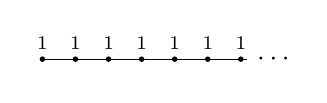
\begin{tikzpicture}[x=.42cm,y=.35cm,baseline=0]
\draw (0,0)--(6.2,0);\foreach \x in {0,...,6}{\fill (\x,0) circle(1pt);\node[above] at (\x,0){\scriptsize $1$};}\node[right]at(6.2,0){$\cdots$};\end{tikzpicture}\\[8pt]
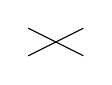
\begin{tikzpicture}[scale=.35,baseline=0]\draw(-1,-.5)--(1,.5) (-1,.5)--(1,-.5);\end{tikzpicture}
& $xy=0$ & $1$ &
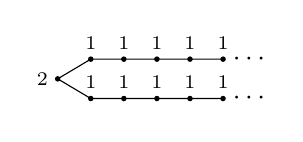
\begin{tikzpicture}[x=.42cm,y=.5cm,baseline=0]
\draw(0,0)--(1,.5)--(5,.5) (0,0)--(1,-.5)--(5,-.5);
\fill(0,0)circle(1pt);\node[left]at(0,0){\scriptsize $2$};
\foreach \y in {-.5,.5}{\foreach \x in {1,...,5}{\fill(\x,\y)circle(1pt);\node[above]at(\x,\y){\scriptsize $1$};}\node[right]at(5,\y){$\cdots$};}\end{tikzpicture}\\[8pt]
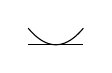
\begin{tikzpicture}[scale=.35,baseline=0]\draw(-1,0)--(1,0);\draw[domain=-1:1]plot(\x,{.6*\x*\x});\end{tikzpicture}
& $y(y-x^2)=0$ & $2$ &
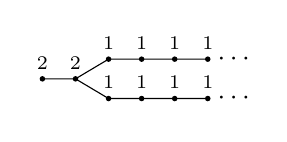
\begin{tikzpicture}[x=.42cm,y=.5cm,baseline=0]
\draw(0,0)--(1,0)--(2,.5)--(5,.5) (1,0)--(2,-.5)--(5,-.5);
\foreach \x in {0,1}{\fill(\x,0)circle(1pt);\node[above]at(\x,0){\scriptsize $2$};}
\foreach \y in {-.5,.5}{\foreach \x in {2,...,5}{\fill(\x,\y)circle(1pt);\node[above]at(\x,\y){\scriptsize $1$};}\node[right]at(5,\y){$\cdots$};}\end{tikzpicture}\\[8pt]
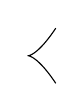
\begin{tikzpicture}[scale=.35,baseline=0]\draw[domain=-1:1,samples=40]plot({\x*\x},{\x*\x*\x});\end{tikzpicture}
& $y^2=x^3$ & $1$ &
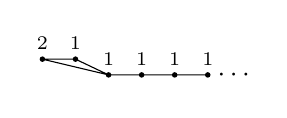
\begin{tikzpicture}[x=.42cm,y=.5cm,baseline=0]
\draw(0,.4)--(1,.4)--(2,0)--(5,0) (0,.4)--(2,0);
\fill(0,.4)circle(1pt);\node[above]at(0,.4){\scriptsize $2$};
\fill(1,.4)circle(1pt);\node[above]at(1,.4){\scriptsize $1$};
\foreach \x in {2,...,5}{\fill(\x,0)circle(1pt);\node[above]at(\x,0){\scriptsize $1$};}\node[right]at(5,0){$\cdots$};\end{tikzpicture}
\end{tabular}
\end{center}
若 $n>2$，\Term{delta-invariant}{$\delta$ 不变量}便不再由此图确定。例如，三条共点且共面的直线之并（分别地，三条不共面的共点直线之并），其\Term{delta-invariant}{$\delta$ 不变量}为 $\delta=3$（分别为 $\delta=2$），而\Term{enriques-diagram}{Enriques 图}相同。我不知道对\Term{unibranch}{单支}\Term{curve}{曲线}是否也会出现这种现象。

下面给出 $n=3$ 时的两个图例，它们不可能出现在平面\Term{curve}{曲线}上（参见 2.5）。依次给出\Term{curve}{曲线}的方程、
\SourcePage{41}
在原点\Term{blow-up}{爆破}后的\Term{strict-transform}{严格变换}的方程、\Term{curve}{曲线}的参数方程、\Term{delta-invariant}{$\delta$ 不变量}，以及\Term{enriques-diagram}{Enriques 图}。
\begin{gather}
\left\{\begin{aligned}y^2&=xz^4,\\z^3&=x^2,\end{aligned}\right.
\qquad
\left\{\begin{aligned}(y/z)^2&=(x/z)^3,\\z&=(x/z)^2,\end{aligned}\right.
\qquad
\left\{\begin{aligned}x&=u^6,\\y&=u^7,\\z&=u^4,\end{aligned}\right.
\qquad \delta=5.\tag{2.25.1}
\end{gather}
\begin{center}
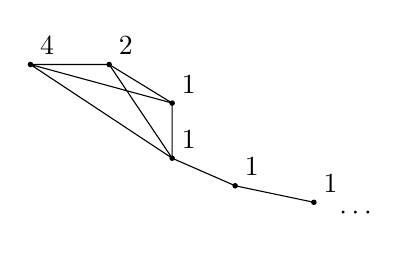
\begin{tikzpicture}[x=1cm,y=.7cm]
\coordinate(a)at(0,0);\coordinate(b)at(1,0);\coordinate(c)at(1.8,-.7);\coordinate(d)at(1.8,-1.7);\coordinate(e)at(2.6,-2.2);\coordinate(f)at(3.6,-2.5);
\draw(a)--(b)--(c)--(d)--(e)--(f);\draw(a)--(c) (a)--(d) (b)--(d);
\foreach \v/\lab in {a/4,b/2,c/1,d/1,e/1,f/1}{\fill(\v)circle(1pt);\node[above right]at(\v){$\lab$};}\node[right]at(3.8,-2.7){$\cdots$};
\end{tikzpicture}
\end{center}
\begin{gather}
\left\{\begin{aligned}y^2z&=x^3,\\z^3&=y^2,\end{aligned}\right.
\qquad
\left\{\begin{aligned}(y/z)^2&=(x/z)^3,\\z&=(y/z)^2,\end{aligned}\right.
\qquad
\left\{\begin{aligned}x&=u^8,\\y&=u^9,\\z&=u^6,\end{aligned}\right.
\qquad \delta=10.\tag{2.25.2}
\end{gather}
\begin{center}
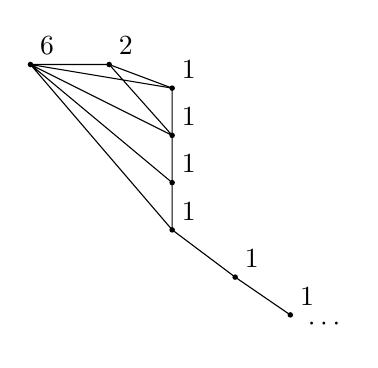
\begin{tikzpicture}[x=1cm,y=.6cm]
\coordinate(a)at(0,0);\coordinate(b)at(1,0);\coordinate(c)at(1.8,-.5);\coordinate(d)at(1.8,-1.5);\coordinate(e)at(1.8,-2.5);\coordinate(f)at(1.8,-3.5);\coordinate(g)at(2.6,-4.5);\coordinate(h)at(3.3,-5.3);
\draw(a)--(b)--(c)--(d)--(e)--(f)--(g)--(h);\draw(a)--(c) (a)--(d) (a)--(e) (a)--(f) (b)--(d);
\foreach \v/\lab in {a/6,b/2,c/1,d/1,e/1,f/1,g/1,h/1}{\fill(\v)circle(1pt);\node[above right]at(\v){$\lab$};}\node[right]at(3.4,-5.5){$\cdots$};
\end{tikzpicture}
\end{center}

\textbf{2.26.} 下述\Term{theorem}{定理} 2.27 在本讲的第一版（由 IHES 散发）中，是作为一个错误的猜想提出的。它在很大程度上得益于与 D. S. Rim 的讨论，并包含了他的一些结果（D. S. Rim，《挠\Term{differential}{微分}与\Term{deformation}{形变}》（\textit{Torsion differentials and deformations}），\Term{theorem}{定理} 2.7 (i)）。
\SourcePage{42}
设 $C$ 是\Term{algebraically-closed}{代数闭}域 $k$ 上的一条\Term{reduced}{约化}\Term{projective-curve}{射影曲线}，$s\in C(k)$。以下记：
\begin{description}
\item[$A_s$：] $C$ 在 $s$ 处的\Term{local-ring}{局部环}（也可用其\Term{completion}{完备化}，这对以下讨论没有区别）；
\item[$\widetilde A_s$：] $A_s$ 的\Term{normalization}{正规化}；
\item[$\delta(s)$：] $\dim_k(\widetilde A_s/A_s)$；
\item[$m_0(s)$：] $\operatorname{Spec}(A_s)$ 的\Term{deformation}{形变}的\Term{formal-versal-scheme}{通用形式概形} $T$ 的\Term{dimension}{维数}。
\end{description}
对 $T$ 的一个\Term{irreducible-component}{不可约分支} $E$，还令 $m_0^E(s)=\dim(E)$。

$\widetilde A_s$ 的\Term{derivation}{导子}模 $\widetilde\tau$ 和 $A_s$ 的\Term{derivation}{导子}模 $\tau$ 都\Term{torsion-free}{无挠}；当 $A_s$ \Term{integral}{整}时，它们都\Term{injectivity}{单射}到 $A_s$ 的\Term{fraction-field}{分式域}的\Term{derivation}{导子}模中；在\Term{generic}{一般}情形，它们都\Term{injectivity}{单射}到 $A_s$ 的\Term{total-ring-of-fractions}{全分式环}（若干个域的积）的\Term{derivation}{导子}模中。此外，借助这些\Term{embedding}{嵌入}，$\tau$ 与 $\widetilde\tau$ \Term{commensurable}{可公度}：$\tau/(\tau\cap\widetilde\tau)$ 和 $\widetilde\tau/(\tau\cap\widetilde\tau)$ 都是\Term{finite-dimensional}{有限维} $k$-\Term{vector-space}{向量空间}。令
\[
m_1(s)=[\widetilde\tau:\tau]
\mathrel{\mathop:}=\dim_k\bigl(\widetilde\tau/(\tau\cap\widetilde\tau)\bigr)
-\dim_k\bigl(\tau/(\tau\cap\widetilde\tau)\bigr).
\]
\begin{SGAresult}{\Term{theorem}{定理}}{2.27}
设 $E$ 是 $A_s$ 的\Term{deformation}{形变}的\Term{formal-versal-scheme}{通用形式概形} $T$ 的一个\Term{irreducible-component}{不可约分支}。若“$A_s$ 在 $E$ 的\Term{generic-point}{一般点} $e$ 上的\Term{deformation}{形变}是\Term{smooth}{光滑}的”，即在 $T$ 上\Term{finite}{有限}的\Term{non-smooth-locus}{非光滑}\Term{form}{形式}\Term{subscheme}{子概形}（由一个 Jacobian \Term{ideal}{理想}定义：第 VI 讲第 5 节）的像不包含 $e$，则
\[
3\delta(s)=m_0^E(s)+m_1(s).
\]
\end{SGAresult}
\SourcePage{43}
\begin{proof}
2.27 是否成立，只依赖于 $A_s$ 的\Term{completion}{完备化}。把 $(C,s)$ 换成在 $s$ 处与其\Term{form}{形式}\Term{isomorphism}{同构}的 $(C',s)$，可设满足下列条件：
\begin{enumerate}
\item[(a)] $s$ 是 $C$ 的唯一\Term{singularity}{奇点}；
\item[(b)] $C$ 没有\Term{infinitesimal-automorphism}{无穷小自同构}。
\end{enumerate}
条件 (b) 保证 $C$ 的\Term{deformation-functor}{形变函子}\Term{prorepresentable}{可 pro 表示}。它甚至是\Term{effective-prorepresentability}{有效地 pro 可表示}的，因为\Term{lifting}{提升} $C$ 上一个给定的（\Term{ample}{丰沛}）\Term{invertible-sheaf}{可逆层}没有\Term{obstruction}{障碍}。设 $f:X_0\to T_0$ 是 $C$ 的\Term{universal-deformation}{普遍形变}，$t_0$ 是 $T_0$ 的\Term{closed-point}{闭点}：$C\xrightarrow{\sim}X_{0t_0}$。

\begin{SGAresult}{\Term{lemma}{引理}}{2.28}
存在 $k$ 上的\Term{finite-type}{有限型}\Term{scheme}{概形} $T_1$、$t_1\in T_1(k)$，以及\Term{proper}{固有}\Term{flat}{平坦}\Term{morphism}{态射} $f:X_1\to T_1$，其在 $t_1$ 处的\Term{fibre}{纤维}为 $C$；并且对任意 $u\in T_1(k)$，$T_1$ 在 $u$ 处的\Term{completion}{完备化}是\Term{fibre}{纤维} $X_{1u}$ 的\Term{formal-moduli-scheme}{形式模概形}。
\end{SGAresult}
下面直接证明这个由 Artin 的\Term{generic}{一般}结果得到的推论。设 $\mathscr L$ 是 $C$ 上的一个\Term{very-ample}{甚丰沛}\Term{invertible-sheaf}{可逆层}，满足 $H^1(C,\mathscr L)=0$，令 $\mathbb P=\mathbb P(H^0(C,\mathscr L))$。有 $v:C\hookrightarrow\mathbb P$。设 $T_2$ 是\Term{hilbert-scheme}{Hilbert 概形}，它分类 $\mathbb P$ 中与 $v(C)\subset\mathbb P$ 有相同 Hilbert \Term{polynomial}{多项式}的\Term{subvariety}{子簇}。设 $t_2\in T_2$ 对应于 $v(C)$。$T_2$ 在 $t_2$ 处的\Term{completion}{完备化} $\widehat T_2$ 在 $S_0$ 上\Term{smooth}{光滑}；$\widehat T_2/T_0$ 的垂直\Term{tangent-bundle}{切丛}由 $T_2$ 的\Term{tangent-bundle}{切丛}的\Term{subbundle}{子丛} $L$ 得到，这个 $L$ 是 $\operatorname{Aut}(\mathbb P)$ 在 $T_2$ 上的\Term{action}{作用}所给出的 $\operatorname{Lie}(\operatorname{Aut}(\mathbb P))$ 的像。在 $t_2$ 的\Term{neighborhood}{邻域}中，取 $n=\dim\operatorname{Aut}(\mathbb P)$ 个方程 $f_1,\ldots,f_n$，使其定义 $T_2$ 的一个经过 $t_2$ 的\Term{subscheme}{子概形} $T'_1$，且其在 $t_2$ 处的\Term{completion}{完备化}在 $T_0$ 上\Term{etale}{平展}。取 $T_1$ 为 $T'_1$ 中 $t_2$ 的一个\Term{neighborhood}{邻域}，使其\Term{tangent-bundle}{切丛}与 $L$ \Term{transverse}{横截}。

\SourcePage{44}
\textbf{2.29.} \Term{functor}{函子}\Term{morphism}{态射}
\[
(C\text{ 的形变})\longrightarrow(A_s\text{ 的形变})
\]
对应于一个\Term{morphism}{态射} $p:T_0\to T$。由第 VI 讲 2.10，$p$ \Term{smooth}{光滑}。设 $t$ 是 $T$ 的\Term{closed-point}{闭点}。$p^{-1}(t)$ 在 $t_0$ 处的 Zariski \Term{tangent-space}{切空间}分类 $C$ 在 $k[\epsilon]$（$\epsilon^2=0$）上的\Term{locally-trivial-deformation}{局部平凡形变}。令 $E_0=p^{-1}(E)$，则
\[
\dim(E_0)=\dim(E)+\dim H^1(C,T^1_{C/k}).\tag{2.29.1}
\]
因为 $X_0/T_0$ \Term{flat}{平坦}，其各\Term{fibre}{纤维}的\Term{arithmetic-genus}{算术亏格} $p$ 相同（$1-p=\chi(\mathcal O)$）。由假设，$E_0$ 的\Term{generic-point}{一般点}处的\Term{fibre}{纤维}\Term{smooth}{光滑}；又因\Term{proper}{固有}\Term{smooth}{光滑}\Term{curve}{曲线}的\Term{formal-moduli-scheme}{形式模概形}是 $3p-3$ 维的\Term{smooth}{光滑}\Term{scheme}{概形}，由 2.28 得
\[
\dim(E)=3p-3.\tag{2.29.2}
\]
设 $\widetilde C$ 是 $C$ 的\Term{normalization}{正规化}，其\Term{arithmetic-genus}{算术亏格}为 $\widetilde p=p-\delta(s)$。有
\begin{align}
\dim H^1(C,T^1_{C/k})&=-\chi(C,T^1_{C/k})\notag\\
&=-\chi(\widetilde C,T^1_{\widetilde C/k})+m_1(s)\notag\\
&=-[3(p-\delta(s))-3]+m_1(s).\tag{2.29.3}
\end{align}
公式 (2.29.1)、(2.29.2)、(2.29.3) 证明了 2.27。
\end{proof}

\begin{SGAresult}{猜想}{2.30}
每条\Term{proper}{固有}\Term{reduced}{约化}\Term{curve}{曲线}都有一个\Term{smooth}{光滑}\Term{deformation}{形变}。
\end{SGAresult}
由 2.27 和 2.28，这个猜想蕴含 $A_s$ 的\Term{deformation}{形变}的\Term{formal-versal-scheme}{通用形式概形}总是\Term{equidimensional}{等维}的，\Term{dimension}{维数}为 $3\delta(s)-m_1(s)$。

\SourcePage{45}
\textbf{2.31.} 设 $C$ 是 $k$ 上的一条\Term{proper}{固有}\Term{reduced}{约化}\Term{curve}{曲线}，其\Term{arithmetic-genus}{算术亏格}为 $p$。以下记：
\begin{description}
\item[$M_0$：] $C$ 的\Term{deformation}{形变}的\Term{formal-versal-scheme}{通用形式概形} $T$ 的\Term{dimension}{维数}；
\item[$M_1$：] $\operatorname{Aut}(C)$ 的 \Term{lie-algebra}{Lie 代数}的\Term{dimension}{维数}。
\end{description}
对 $T$ 的一个\Term{irreducible-component}{不可约分支} $E$，以 $M_0^E$ 表示 $E$ 的\Term{dimension}{维数}。

2.27 的整体对应结果如下。
\begin{SGAresult}{命题}{2.32}
若 $C$ 在 $E$ 的\Term{generic-point}{一般点}上的\Term{deformation}{形变}是\Term{smooth}{光滑}的，则
\[
3p-3=M_0^E-M_1.
\]
\end{SGAresult}
\begin{proof}
设 $X\subset C(k)$ 是 $C$ 的一个\Term{finite}{有限}\Term{smooth-point}{光滑点}集，使得 $C$ 上在每个 $x\in X$ 处为零的\Term{vector-field}{向量场}必为零。$(C,X)$ 的\Term{deformation-functor}{形变函子}\Term{prorepresentable}{可 pro 表示}，且满足 2.28 的一个变式。$(C,X)$ 的\Term{formal-moduli-scheme}{形式模概形}在 $T$ 上\Term{smooth}{光滑}，\Term{relative-dimension}{相对维数}为 $\#X-M_1$；由 2.28 的对应结果，得到
\[
M_0+(\#X-M_1)=3p-3+\#X,
\]
从而得 2.32。
\end{proof}
设 $k$ 的\Term{characteristic-field}{特征}为 $0$。这时 $M_1=\dim\operatorname{Aut}(C)$。下面给出 $m_1(s)$ 的类似解释。

\SourcePage{46}
\begin{SGAresult}{\Term{lemma}{引理}}{2.33}
若 $k$ 的\Term{characteristic-field}{特征}为 $0$，则 $A_s$ 的每个\Term{derivation}{导子}都延拓为 $\widetilde A_s$ 的一个\Term{derivation}{导子}。
\end{SGAresult}
\begin{proof}
若 $D$ 是 $A_s$ 的一个\Term{derivation}{导子}，则 $\exp(Dt)=\sum D^nt^n/n!$ 是 $A_s\otimes_k k[t]$ 在 $(s,0)$ 处的\Term{completion}{完备化}的一个\Term{automorphism}{自同构}。由\Term{transport-of-structure}{结构搬运}，这个\Term{automorphism}{自同构}\Term{action}{作用}于该环的\Term{normalization}{正规化} $(\widetilde A_s\otimes k[t])^{\wedge}$。模 $t^2$ \Term{reduced}{约化}，得到 $\widetilde A_s^{\wedge}\otimes_k k[t]/(t^2)$ 的一个\Term{automorphism}{自同构} $1+Dt$，从而 $D$ 延拓为 $\widetilde A_s^{\wedge}$ 的一个\Term{derivation}{导子}。由于它也延拓到 $A_s$ 的\Term{fraction-field}{分式域}（当 $A_s$ 非\Term{integral}{整}时，取\Term{total-ring-of-fractions}{全分式环}），故它延拓到 $\widetilde A_s$。
\end{proof}
设 $s$ 为\Term{singularity}{奇点}。类似的论证说明，$D$ 所定义的 $\operatorname{Spec}(\widetilde A_s)$ 上的\Term{vector-field}{向量场}在 $s$ 上方的每一点处都为零。

设 $\mathfrak c$ 是 $\widetilde A_s$ 的一个\Term{ideal}{理想}，包含在 $\widetilde A_s/A_s$ 的\Term{conductor}{导子理想}中。设 $\widetilde G_{\mathfrak c}=\operatorname{Aut}(\widetilde A_s/\mathfrak c)$，$G_{\mathfrak c}$ 为 $\widetilde G_{\mathfrak c}$ 中\Term{stable}{稳定}\Term{subalgebra}{子代数} $A_s/\mathfrak c$ 的\Term{subgroup}{子群}。对 $\mathfrak d\subset\mathfrak c$，$\widetilde G_{\mathfrak d}$ \Term{stable}{稳定} $\mathfrak c/\mathfrak d$，并\Term{surjectivity}{满射}到 $\widetilde G_{\mathfrak c}$（注意，若 $t$ 是一个\Term{uniformizer}{一致化参数}，则 $g\in\widetilde G_{\mathfrak c}$ 由 $g(t)$ 确定，而 $g(t)$ 可以是任意\Term{uniformizer}{一致化参数}）。因此，带\Term{base-point}{基点}的\Term{homogeneous-space}{齐性空间} $\widetilde G_{\mathfrak c}/G_{\mathfrak c}$ 与 $\mathfrak c$ 无关，记作 $\widetilde G/G$。

以 $\widetilde\tau_0$ 表示 $\operatorname{Spec}(\widetilde A_s)$ 上在 $s$ 上方各点处都为零的\Term{vector-field}{向量场}所成的 $\widetilde A_s$-模。对\Term{singularity}{奇点} $s$，有
\[
\dim_k(\widetilde\tau/\widetilde\tau_0)=\text{分支数};
\]
\[
\widetilde\tau_0/\tau\simeq\widetilde G/G\text{ 在原点处的切空间}.
\]
\SourcePage{47}
\begin{SGAresult}{命题}{2.34}
当\Term{characteristic-field}{特征}为 $0$、$s$ 为\Term{singularity}{奇点}时，整数 $m_1(s)$ 等于\Term{branch}{分支}数与 $\widetilde G/G$ 的\Term{dimension}{维数}之和。
\end{SGAresult}

\SGAsection{}{参考文献}
\begin{description}
\item[{[1]}] P. Defrise，《\Term{algebra}{代数}\Term{surface}{曲面}间有理对应的\Term{local-scheme}{局部}研究》（\textit{Étude locale des correspondances rationnelles entre surfaces algébriques}），资格论文，布鲁塞尔，1949。
\item[{[2]}] P. Deligne、D. Mumford，《给定\Term{genus}{亏格}的\Term{curve}{曲线}\Term{space}{空间}的\Term{irreducibility}{不可约性}》（\textit{The irreducibility of the space of curves of a given genus}），\textit{Publ. Math. IHES} \textbf{36}（1969），第 75--110 页。
\item[{[3]}] Enriques、Chisini，《方程与\Term{algebra}{代数}函数的几何理论讲义》（\textit{Lezioni sulla teoria geometrica delle equazioni et delle funzioni algebriche}），Zanichelli 出版社，博洛尼亚，1924。
\item[{[4]}] R. Hartshorne，《\Term{residue}{留数}与\Term{duality}{对偶性}》（\textit{Residues and duality}），\textit{Lecture Notes in Math.} \textbf{20}，Springer，1966。
\item[{[5]}] S. Lichtenbaum，《\Term{discrete-valuation-ring}{离散赋值环}上的\Term{curve}{曲线}》（\textit{Curves over discrete valuation rings}），\textit{Am. J. of Math.} \textbf{15}，第 2 期，1968 年 4 月，第 380--405 页。
\item[{[6]}] I. Manin，《\Term{perfect-field}{完美域}上的有理\Term{surface}{曲面}》（\textit{Rational surfaces over perfect fields}），\textit{Publ. Math. IHES}，第 30 号，第 55--114 页。
\item[{[7]}] D. Mumford，《\Term{algebra}{代数}\Term{surface}{曲面}的\Term{normal}{正规}\Term{singular-point}{奇点}的\Term{topology}{拓扑}与一个单\Term{purity}{纯性}判据》（\textit{The topology of normal singularities of an algebraic surfaces and a criterion for simplicity}），\textit{Publ. Math. IHES}，第 9 号，第 5--22 页。
\item[{[8]}] A. Néron，《\Term{local-field}{局部域}与整体域上\Term{abelian-variety}{阿贝尔簇}的\Term{minimal-model}{极小模型}》（\textit{Modèles minimaux des variétés abéliennes sur les corps locaux et globaux}），\textit{Publ. Math.}，第 21 号。
\end{description}
\SourcePage{48}
\begin{description}
\item[{[9]}] M. Raynaud，《\Term{picard-functor}{Picard 函子}的\Term{specialization}{特殊化}。\Term{representability}{可表示性}的数值判据》（\textit{Spécialisation du foncteur de Picard. Critères numériques de représentabilité}），\textit{CR Acad. Sci. Paris}，第 264 卷，第 1001--1004 页，1967 年 6 月。
\item[{[10]}] Saint-Donat，《关于 G. Castelnuovo 和 F. Enriques 的一个\Term{theorem}{定理}》（\textit{Sur un théorème de G. Castelnuovo et F. Enriques}），第三阶段博士论文，里昂。
\item[{[11]}] O. Zariski，《由无穷邻近\Term{base-point}{基点}定义的\Term{polynomial}{多项式}\Term{ideal}{理想}》（\textit{On polynomial ideals defined by infinitely near base points}），\textit{Am. J. Math.}，第 60 卷，1938，第 151 页。
\item[{[12]}] D. G. Northcott，《关于平面\Term{curve}{曲线}的\Term{genus}{亏格}公式》（\textit{On the genus formula for plane curves}），\textit{J. London Math. Soc.} \textbf{30}，1955，第 376--382 页。
\item[{[13]}] D. G. Northcott，《抽象\Term{blow-up}{爆破}与无穷\Term{proximate-point}{邻近点}》（\textit{Abstract dilatations and infinitely near points}），\textit{Proc. Cambridge Philos. Soc.} \textbf{52}，1956，第 178--197 页。
\end{description}
“\Term{infinitely-near-point}{无穷邻近的点}”这一概念，在下书第二章由 Lipman 撰写的附录中有所讨论：
\begin{description}
\item[{[14]}] O. Zariski，《\Term{algebra}{代数}\Term{surface}{曲面}》（\textit{Algebraic surfaces}），\textit{Ergebnisse} \textbf{61}，Springer Verlag。
\end{description}
